\documentclass[10pt,a4paper]{scrartcl}
\usepackage[utf8]{inputenc}
\usepackage[german]{babel}
\usepackage[T1]{fontenc}
\usepackage{amsmath}
\usepackage{amsfonts}
\usepackage{amssymb}
\usepackage{lmodern}
\usepackage{threeparttable}
\usepackage{listings}
\usepackage{color}
\usepackage[german]{struktex}
\usepackage[usenames,dvipsnames,svgnames,table]{xcolor}
\usepackage[all]{xy}
\definecolor{hellrot}{HTML}{A21717}
\usepackage{graphicx}
\usepackage{pgfplots}
%\usepackage{epstopdf}
\usepackage[colorlinks=true,linkcolor={hellrot}]{hyperref}
\usepackage[left=2cm,right=2cm,top=2cm,bottom=2cm]{geometry}
\usepackage{array}
\newcolumntype{C}[1]{>{\centering}p{#1}} 
\definecolor{lightblue}{RGB}{25,33,132}
\definecolor{middlegray}{RGB}{100,100,100}
\definecolor{dkgreen}{RGB}{1, 50, 32}
\lstset{   language=Delphi,
           numbers=left,
           numberstyle=\tiny,
           stepnumber=1,
           numbersep=9pt,
           % backgroundcolor=\color{listingbackground},
           basicstyle=\scriptsize,
           captionpos=b,
           breaklines=true,
           breakindent=20pt,
           texcl=true,
           % mathescape=true,
           escapechar=•,  % ASCI Char #263 (als ALT+263 auf dem Numpad eingeben)
           xleftmargin=0pt,
           % escapebegin=$,
           % escapeend=$,
           extendedchars=true,
           float=false,
           frame=none,
           rulesepcolor=\color{black},
           rulesep=2pt,
           framesep=3pt,
           framexleftmargin=3pt,
           framexrightmargin=3pt,
           columns=[c]fixed,
           basewidth={0.6em,0.45em},
           fontadjust=false,
           commentstyle=\color{middlegray}\ttfamily,
           keywordstyle=\bfseries\ttfamily\color{lightblue}
        }

\author{TEAM \glqq{}Der LAMABÄR\grqq{}}
\date{\today}
\title{34. Bundeswettbewerb Informatik\\3. Aufgabe}
\subtitle{Dokumentation}
\begin{document}
\maketitle
\tableofcontents
\section{Lösungsidee}
Im Wesentlichen zielt diese Aufgabe darauf ab einen Algorithmus zu finden, der für eine beliebige natürliche Zahl alle möglichen Darstellungen der Selben als Summe finden soll. Es gibt dabei nur zwei Einschränkungen: Die Anzahl der Summanden ist in dem Fall die Anzahl der Behälter und die maximale Größe eines jeden Summanden entspricht dem maximalen Fassungsvermögen des dazugehörigen Behälters.\\
Die Aufgabe alle möglichen Kombinationen für sieben Flaschen und zwei Behältern mit einem Fassungsvermögen von drei und fünf kann man also auch folgendermaßen darstellen:
\begin{itemize}
\item 7=3+4
\item 7=2+5
\end{itemize}
In der Informatik wird dieses Problem als Paritionierungsproblem bezeichnet.\\

Die Idee meines Algorithmus besteht im Wesentlichen darin, dass ein baumähnlicher, gerichteter Graph erzeugt wird und das \glqq{}Backtracking\grqq{}-Verfahren daran angewandt wird, also jeder mögliche Pfad bzw. in dem Fall Kombination rekursiv durchgegangen wird und der Wert eines jeden einzelnen Knoten einer gerade durchlaufenden Kombination dabei summiert wird. Dabei gibt es in jeder \glqq{}Stufe\grqq{} des Baumes, welche einem Behälter entspricht, so viele Knoten, wie Flaschen in den jeweiligen Behälter passen. Die Knoten auf jeder Stufe sind von 0 bis maximales Fassungsvolumen des Behälters durchnummeriert; Diese Zahl entspricht dem Wert des Knotens. Jeder Knoten zeigt, sofern es nicht der letzte Behälter ist, auf alle Knoten des nächsten Behälter, sodass man durch die Backtracking Methode alle möglichen Kombinationen \glqq{}errechnen\grqq{} kann. Die Anzahl der Flaschen ist für die Erzeugung des Graphen irrelevant, da es nur bei der Rekursion benötigt wird, um zu überprüfen, ob der Wert einer Kombination der Anzahl an Flaschen entspricht oder nicht.\\
Dazu ein Beispiel. Es gibt drei Behälter mit einem Fassungsvolumen von je eins, drei und vier Flaschen. In der \autoref{fig:gerichtet} ist der daraus entstehende Graph zu diesem Beispiel skizziert.\\
\begin{figure}[!hbtp]%
  \caption{beispielhafter Graph}
  \label{fig:gerichtet}
  \begin{displaymath}
    \xymatrix{
     & & & & \bullet Root \ar@/_/[dll] \ar@/^/[drr]                 \\
     Behälter 1: & & \bullet 0 \ar@/_/[dl] \ar@/_/[dr] \ar@/_/[drrr] \ar@/_/[drrrrr] & & & & \bullet 1 \ar@/^/[dr] \ar@/^/[dl] \ar@/^/[dlll] \ar@/^/[dlllll] & \\
     Behälter 2: & \bullet 0 \ar@/_/[dr] \ar@/_/[drrr] \ar@/_/[drrrrr] & & \bullet 1 \ar@/^/[dl] \ar@/_/[dr] \ar@/_/[drrr] & & \bullet 2 \ar@/^/[dlll] \ar@/^/[dl] \ar@/_/[dr] & & \bullet 3 \ar@/^/[dlllll] \ar@/^/[dlll] \ar@/^/[dl] \\
     Behälter 3: & & \bullet 0 & & \bullet 1 & & \bullet 2 &          }\\
  \end{displaymath}
\end{figure}

Der logische Ablauf des rekursiven Algorithmus, der jede mögliche Kombination durchläuft, ist in der \autoref{fig:Nassi} dargestellt. Wie der gerichtete Graph erstellt wurde, wird im \hyperlink{section.2}{2. Kapitel} näher erläutert, da es kein Bestandteil der Idee ist.\\
\begin{figure}[!hbtp]%
  \caption{Nassi-Shneiderman-Diagramm zum Paritionierungsproblem}
  \label{fig:Nassi}
	\begin{centernss}
		%\sProofOn
		\begin{struktogramm}(160,143)[procedure Paritionierung(rootKnoten,wert,stufe:\pVar{int})]
			\renewcommand{\pLanguage}{Pascal}
			\assign%
			{
			\begin{declaration}[wichtige Variablen:]
				\description{\(FBehälterarray\)}{Ein dynamisches \pVar{Array}, in der für jeden Behälter das Fassungsvermögen angegeben ist}
				\description{\(FFlaschenanzahl\)}{}
				\description{\(FBehälteranzahl\)}{}
				\description{\(FmaxFlaschenInputproBehälter\)}{\pVar{Array}: Gibt an, wie viele Flaschen noch in die Behälter, die unter dem i-ten behälter sind, hineinpassen}
			\end{declaration}
			}
		\ifthenelse[15]{3}{1}{wert = FFlaschenanzahl}{\sTrue}{\sFalse}
			\assign{\(Zähler \gets Zähler+1\) \pComment{ // Kombination gefunden}}
			\exit{ \pComment{Braucht nicht mehr weiterzusuchen.}}
			\change
		\ifend
		\ifthenelse[15]{3}{1}{wert > FFlaschenanzahl}{\sTrue}{\sFalse}
			\exit{Exit \pComment{ // keine Kombination in diesem Zweig mehr möglich}}
			\change
		\ifend
		\ifthenelse[15]{3}{1}{FmaxFlaschenInputproBehälter[stufe]+wert < FFlaschenanzahl}{\sTrue}{\sFalse}
			\exit{Exit \pComment{ // keine Kombination in diesem Zweig mehr möglich}}
			\change
		\ifend
		\dfr
		\assign{starte für jeden Zeiger, ausgehend vom aktuellen rootKnoten, folgenden Code (rekursiv):}
		\sub{Paritionierung(aktuell ausgewählter Zeiger vom rootKnoten, Wert des Knotens auf den der Zeiger zeigt + aktuellen Wert)}
		\dfrend

		\end{struktogramm}
	\end{centernss}
\end{figure}
\\
\subsection{Laufzeitkomplexität}
Ich habe mich hier für den Algorithmus des \glqq{}Backtrackings\grqq{} und nicht für die \glqq{}Tiefensuche\grqq{} entschieden, da ersteres effizienter ist, da erkannt wird, wenn eine weitere Berechnung an einem bestimmten Knoten nicht mehr sinnvoll ist, da keine Lösung mehr möglich ist, wenn z.B. der errechnete Wert größer als die Anzahl der Flaschen ist. Mein Algorithmus wurde außerdem insoweit optimiert, als dass er merkt, dass das Weiterrechnen von einem bestimmten Knoten aus nicht mehr sinnvoll ist, da der Wert zu niedrig ist, als dass es noch zu einer Lösung kommen kann. Dazu gibt es ein Array, in dem für jede Stufe, also für jeden Behälter, genannt wird, wie viele Flaschen maximal in den unter mir liegenden Behältern noch hineinpassen würden. Diese beiden Optimierungen verändern allerdings leider nichts an der Tatsache, dass die Ordnung dadurch nicht verändert wird. Zur Ermittlung der Ordnung habe ich einmal den BestCase in der
\autoref{eq:BestCase} und den WorstCase in der 
\autoref{eq:WorstCase} und
\autoref{eq:WorstExpoCase} ermittelt.\\
\begin{align}
	Pfadanzahl=1 \label{eq:BestCase}
\end{align}
Zur Erläuterung: Im besten Fall haben wir genau null Flaschen oder genau so viele Flaschen, wie die Summe der Fassungsvermögen aller Behälter ist, die maximale Anzahl an Flaschen, da hier einer der beiden Optimierungen greifen, und haben dementsprechend eine Ordnung 1, wenn wir uns auf die Anzahl der Pfade beziehen, da alle anderen Pfade durch die \glqq{}Backtracking\grqq{}-Methode nicht betreten werden. Also gilt $\mathcal{O} {(1)}$.\\
 Der WorstCase wäre der Fall, wenn die Flaschenanzahl genau die Hälfte der Summe der Fassungsvermögen aller Behälter ist. Dann würden beide Optimierungen nur teilweise greifen und am geringsten Bewirken, da sie nur bei geringen oder hohen Flaschenanzahlen sehr wirksam sind. \\ \textit{i}=Fassungsvermögen eines speziellen Behälters; $\textit{V}_{i}$=Volumen des \textit{i}-ten Behälters; \textit{n}=Anzahl der Behälter:
\begin{align}
	Pfadanzahl=\dfrac{\prod\limits_{i=1}^{n} (a_{i}+1)}{2} \label{eq:WorstCase}
\end{align}
Der Term mit der Produktformel setzt sich mit der Annahme auseinander, dass die letzte Optimierung nicht greift und der WorstCase der Fall ist, und die maximal mögliche Flaschenanzahl der schlimmste Fall wäre. Dann wäre der Average-Fall die obengenannte Formel, welche mit beiden Optimierungen nun mal der schlimmste Fall ist. \\
Der exponentielle Zusammenhang wird durch einen Spezialfall deutlich: Alle Behälter n haben das gleiche Fassungsvermögen V:
\begin{align}
	Pfadanzahl=\dfrac{n^{V+1}}{2} \label{eq:WorstExpoCase}
\end{align}
Im WorstCase gilt also $\mathcal{O} {(n^{x})}$. Genau bei dieser Laufzeitanalyse sieht man den Vorteil des \glqq{}Backtrackings\grqq{} gegenüber der \glqq{}Tiefensuche\grqq{}, da selbst im WorstCase durch die Optimierungen erstere effizienter ist als letztere und - abgesehen von den beiden einfachen ressourcenunbelastenden If-Abfrage, ob die Flaschenanzahl größer als der aktuell errechnete Wert ist bzw. eine Lösung aufgrund einer zu geringen Flaschenanzahl an der aktuellen Position mehr möglich ist, die schließlich bei jeder Rekursionstiefe durchgeführt wird - in jeden anderen Fall ist die Rechenleistung deutlich humaner und man könnte z.B. auch fünf Behälter mit je 300 Fassungsvermögen bei nur zwei Flaschen bzw. 288 Flaschen in einer akzeptablen Zeit lösen.\\

Nichtsdestotrotz besteht hier ein exponentieller Zusammenhang (s. \hyperlink{section.3}{Beispiele}), was mit der Komplexitätsklasse des Paritionierungsproblems (NP-vollständig) übereinstimmt, was impliziert, dass es keinen effizienteren Algorithmus mit z.B. $\mathcal{O} {(n)}$ oder gar $\mathcal{O} {(\log{n})}$ gibt. Jegliche Verbesserung des Codes würde die Steigung der exponentielle Funktion nur um ein Faktor verringern, sie kann jedoch nicht das exponentielle Wachstum verhindern.\\

Meine Laufzeitanalyse geht in dem Fall nur auf die Anzahl der durchlaufenden Pfade ein, jedoch nicht auf die Anzahl der durchlaufenden Knoten, was durchaus aussagekräftiger wäre, da bei einem unausbalancierten Graphenbaum es mehr Pfade gibt als Knoten durchlaufen werden; bei einem ausbalancierten Graphenbaum werden jedoch weitaus mehr Knoten bei der gleichen Pfadanzahl durchlaufen. In dem Fall würde der zusätzliche Rechenaufwand die Anzahl der Knoten zu berechnen, was die Komplexität der Formel deutlich erhöhen würde, nicht im Einklang mit dem Nutzen stehen. Dieser ist nämlich nicht ein exaktes Ergebnis zu bekommen, sondern eine sehr gute Näherung, was die Pfadanzahl durchaus angibt.

Als einen weiteren Optimierungsfaktor, der allerdings erst bei der Betrachtungsweise mit den durchlaufenden Knoten deutlich wird und daher nur exemplarisch und nicht durch eine Formel gezeigt werden kann, ist die Sortierung nach Fassungsvermögen der Behälter vor der eigentlichen Rekursion. Hierbei stellt sich die Frage, was effizienter ist: Aufsteigend oder absteigend oder ob für die Beantwortung dieser Frage die Flaschenanzahl in Relation zu dem maximalen Fassungsvermögen aller Behälter eine Rolle spielt oder nicht. \\
Dazu einmal ein exemplarischer Graph mit drei Behältern mit einem Fassunsgvermögen von je 2, 3 und 4:
\begin{center}
	\begin{tikzpicture}
		\begin{axis}[ymin=0,
			width=0.7\textwidth,height=0.3\textheight,
			title={Anzahl der durchlaufenen Knoten bei 4-3-2 \& 2-3-4 Sortierung},
			xtick={1,2,3,4,5,6,7,8,9},
			xlabel={Flaschenanzahl},
			extra y ticks={13,50,66},	
			extra y tick labels={{13},{50},{66}},
			extra y tick style={grid=major,
				tick label style={xshift=-0.1cm}},
			ylabel={Knotenanzahl},
			legend entries={4-3-2,2-3-4}, 
			legend style={at={(1,1)},xshift=0.2cm,anchor=north west,nodes=right},
			enlarge x limits=0]
			\addplot table[x index={0}, y index={1}] {Laufzeitanalyse.txt};
			\addplot table[x index={0}, y index={2}] {Laufzeitanalyse.txt};
		\end{axis}
	\end{tikzpicture}
	\captionof{figure}{Abhängigkeit der Sortierung bei der Laufzeit}
	\label{fig:Sortierung}
\end{center}
Was man aus dem Graphen exemplarisch erkennen kann, ist zum einen, dass sich meine Annahme zum WorstCase sich bestätigt hat (dieser ist bei der Hälfte von der Summe aller Fassungsvermögen). Zum Zweiten, dass die Angabe der Pfadanzahl nur ungenau ist, da es auf die Reihenfolge der Behälter ankommt und sich so eine Amplitude von bis zu 18 Knoten in diesem Fall bildet. Zum Letzteren, dass die Sortierung 4-3-2 effizienter ist, was allerdings mit meinen Optimierungen zusammenhängt, da ohne die letzte Optimierung (Erkennung eines zu niedrigen Wertes, als dass man fortfahren könnte und noch ein Ergebnis finden könnte) beide Methoden sich nichts tun. Offensichtlich ist die 4-3-2 Sortierung in den Bereichen effizient, wo die anderen beiden Optimierungen, die in der Rekursion mittels If-Clauses verwendet werden, ineffizient sind. In den Bereichen, wo die 4-3-2 Sortierung ineffizient ist, macht das nichts, da da die beiden Optimierungen greifen.


\section{Umsetzung}
Für die Umsetzung habe ich das Modell-View-Controller(MVC)-Prinzip verwendet, wobei ich View und Controller der Einfachheit halber zu einer Instanz vereint habe. Hinzu kommt eine objektorientierte Programmierung. Von dem View-Controller werden die Flaschenanzahl, Behälteranzahl und das Volumen eines jeden Behälters über die Konsole abgefragt und mit den Werten ein Objekt der Klasse TBaum erzeugt. Diese erstellt auch sogleich den gerichteten Graphen. Danach führt der Benutzer die Procedure \glqq{}parition\grqq{} aus, welche dann wiederum die Rekursion ausführt. Nach dem Durchlauf der Rekursion wird durch den aufgerufenen Getter \glqq{}getzaehler\grqq{} die Anzahl aller möglichen Kombinationen in der Konsole ausgegeben. Das Objekt TBaum greift dafür auf die Klasse TKnoten zurück, um alle Knoten des Baumes zu erzeugen. Für jeden Knoten wird ein Objekt der Klasse TKnoten erstellt, welche dann in einem dynamischen Array des Typs TKnoten gespeichert werden. Jedes Objekt der Klasse TKnoten hat einen Wert (z.B. 4 Flaschen) und ein oder mehrere Zeiger auf seine \glqq{}Kinder\grqq{}, also auf die Knoten, die dem nächsten Behälter zugehörig sind. Gibt es keinen nächsten Behälter, so bleibt diese Variable leer. Zur Veranschaulichung kann das UML-Diagramm in \autoref{fig:UMLDiagramm} verwendet werden.\\
\begin{figure}
	\centering
	\caption{UML-Diagramm der Klasse TBaum und TKnoten}
	\label{fig:UMLDiagramm}
	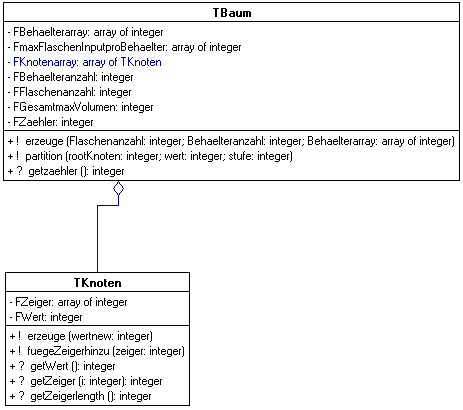
\includegraphics[]{UML.png}
\end{figure}

Im \hyperlink{section.1}{1. Kapitel} habe ich bereits den eigentlichen Algorithmus, also die Rekursion, beschrieben, es fehlte aber noch der Algorithmus, der den Baum erstellt. Dazu habe ich noch ein Nassi-Shneidermann-Diagramm in \autoref{fig:erstNassi} erstellt. Der Algorithmus besteht im Wesentlichen aus zwei Elementen. Nachdem der Root-Knoten erzeugt wurde, wird für jeden Behälter erst einmal die entsprechenden Knoten von dem derzeitigen Behälter nach dem Prinzip aus \autoref{fig:gerichtet} erstellt. Dann werden im zweiten Schritt für alle Knoten des vorherigen Behälters Zeiger auf die Knoten im aktuellen Behälter erstellt. Dies wird dann für jeden Behälter wiederholt. Mit diesem Prinzip macht man also aus einem Graphen ein Array mit Knoten, die man nur durch das Inspizieren aller Knoten wieder zurück in den Graphen einordnen kann, da jeder Knoten nur die Information enthält, welche Knoten unter dem jeweiligen Knoten sind. Mehr Informationen werden aber auch nicht für das \glqq{}Backtracking\grqq{} benötigt, sodass Speicher durch das Wegfallen unnötiger Informationen gespart werden kann.

\begin{figure}[!hbtp]%
  \caption{Nassi-Shneiderman-Diagramm zur Erstellung des gerichten Graphens}
  \label{fig:erstNassi}
	\begin{centernss}
		%\sProofOn
		\begin{struktogramm}(170,151)[constructor erzeuge(Flaschenanzahl, Behälteranzahl:\pVar{int}; Behälterarray: \pVar{array} of \pVar{int})]
			\renewcommand{\pLanguage}{Pascal}
			\assign%
			{
			\begin{declaration}[wichtige Variablen:]
				\description{\(Behälterarray\)}{s. \autoref{fig:Nassi}}
				\description{\(Flaschenanzahl\)}{}
				\description{\(Behälteranzahl\)}{}
				\description{\(Knotenarray\)}{Ein dynamisches \pVar{Array} vom Typ \pVar{TKnoten}, welcher alle Knoten beinhaltet. Der Index ist dabei die eindeutige Zuordnung zu einem bestimmten Knoten.}
			\end{declaration}
			}
		\assign {Knotenarray[0]:=TKnoten.erzeuge(0) \pComment{ // Erzeuge Wurzel}}
		\dfr
			\assign{für I:=1 bis Behälteranzahl tue:}
			\dfr
				\assign{für J:=0 bis Behälterarray[i] tue:}
				\sub{setlength(Knotenarray,length(Knotenarray)+1) \pComment{ // erweitere das dynamische Array um einen Wert}}
				\sub{Knotenarray[length(Knotenarray)-1]:=TKnoten.erzeuge(j) \pComment{ // und erzeuge einen neuen Knoten}}
			\dfrend
			\dfr
				\assign{für J:=0 bis Behälterarray[i-1] tue:}
				\dfr
					\assign{für K:=0 bis Behälterarray[i] tue:}
					\sub{Knotenarray[length(Knotenarray)-j-Behaelterarray[i]-2].addZeiger(length(Knotenarray)-k-1) \pComment{ // Füge jedem \glqq{}Vater\grqq{} des aktuellen Knotens einen Verweis auf dem derzeitigen Knoten zu}}		
				\dfrend
			\dfrend
		\dfrend
		\end{struktogramm}
	\end{centernss}
\end{figure}
\section{Beispiele}
Als Programmeingabe gibt es nur, wie es auch in der Aufgabenstellung und in den Beispielen vorgegeben wurde, die Flaschenanzahl, die Anzahl der Behälter und daraus resultierend die Anzahl von jedem Behälter. Danach wird das Programm gestartet. Da es hier außer den bereits beschriebenen Phänomen bedingt durch meine Laufzeitoptimierungen (s. \autoref{fig:Sortierung}) keine besonderen \glqq{}Randbeispiele\grqq{}, \glqq{}Sonderfälle\grqq{} oder ähnliches gibt und auch selbst erdachte Beispiele genauso viel Sinn ergeben wie die Verwendung der vorgegebenen Beispiele, werde ich im Folgenden nur solche Beispiele auflisten.\\
Ab dem dritten Beispiel dauerte die Berechnung zu lange, als dass ich die Anzahl der Kombinationen ausrechnen könnte. Bei Beispiel 4 und 5 würde es aufgrund der noch größeren Anzahl der durchlaufenen Knoten, noch länger dauern, weshalb ich das Ergebnis hier nicht aufgeführt habe.
\subsection{Beispieltabelle}
	\begin{center}
	\begin{threeparttable} 
	\begin{large}
	\renewcommand{\arraystretch}{1.5}
	\caption{Beispiele}
		\begin{tabular}{|c||C{1.7cm}|C{1.7cm}|C{4cm}||C{2.5cm}|C{3.5cm}|}
			\hline
			& Flaschen-anzahl & Behälter-anzahl & Fassungsvermögen der i-ten Behälter & Kombinations-anzahl & Anzahl der durchlaufenen Knoten \tabularnewline 
			\hline \hline
			Beispiel 0 & 7 & 2 & \{3, 5\} & 2 & 15 \tabularnewline 
			\hline
			Beispiel 1 & 5 & 3 & \{2, 4, 4\} & 13 & 58 \tabularnewline 
			\hline
			Beispiel 2 & 10 & 3 & \{5, 8, 10\} & 48 & 336 \tabularnewline 
			\hline
			Beispiel 3 & 30 & 20 & \{1, 2, 3, 4, 5, 6, 7, 8, 9, 10, 11, 12, 13, 14, 15, 16, 17, 18, 19, 20\} & {\O}  & 22412157560166 \tabularnewline 
			\hline
		\end{tabular}
		\label{tab:meinetabelle}
	\end{large}
	\end{threeparttable} 
	\end{center}
\section{Quelltext}
Im Folgenden werden die beiden zentralen Quelltexte, die Rekursion und die Erzeugung des gerichteten Graphens, wie sie auch schon in den beiden Nassi-Sneiderman-Diagrammen dargestellt wurden (\autoref{fig:Nassi} und \autoref{fig:erstNassi}), dargelegt. Da der restliche Code entweder für die Kommunikation zwischen den Klassen (Getter, Setter und Constructor) oder für die grafische Aufbereitung inklusive das vorherige Erkennen von falschen Eingaben von dem Benutzer zuständig ist, wäre es nicht sinnvoll, diesen hier zu integrieren, da diese Komponente die eigentliche Lösungsfindung nicht beeinflusst.
\subsection{Erzeugung des gerichteten Graphen}
\lstinputlisting[language=Delphi, firstline=31, lastline=65,caption={Erzeugung eines gerichteten Graphen in Turbo Pascal}]{../uBaum.pas}
\subsection{Rekursion}
\lstinputlisting[language=Delphi, firstline=67, lastline=78,caption={Rekursion in Turbo Pascal}]{../uBaum.pas}


\listoffigures
\end{document}